




\subsection{Influence of (non)-linear material parameters}


The influence of linear/non-linear material parameters were investigated by pressurizing both bellows equally for 20kPa and 80kPa for both linear and non-linear material parameters. For the linear case a Young's modulus ($E$) of 69 Mpa and a Poisson ratio ($\nu$) of 0.45 were used. These parameters can be used to calculate the Lamé parameters necessary to simulate non-linear Neo-Hookeon deformation. To this end, Lamé's first parameter or shear modulus $\mu$ and bulk modulus $\kappa$ need to be calculated, these can be calculated with the following equations, respectively

\begin{equation}
    \mu = \frac{E}{2(1+\nu)}
\end{equation}


\begin{equation}
    \kappa = \frac{E}{3(1-2\nu)}
\end{equation}

In the Abaqus FEM environment these constants need to be translated to \verb+C10+ and \verb+D1+ parameters by the with

\begin{equation}
    \verb+C10+ = \frac{\mu}{2}
\end{equation}


\begin{equation}
    \verb+D1+ = \frac{2}{\kappa}
\end{equation}

As mentioned, two simulations were carried out pressurizing both bellows equally for 20kPa and 80kPa.Deformations in $x,y,z$ direction for both material parameters are shown in Table (\ref{tab3:linnonlindef}). The procedure to calculate deformation works as follows. After the bellows are pressurized, the nodes in the top plate are isolated. Hereby, we assume that the connection plate at the tip of the robot does not deform when pressurizing the bellows. In Matlab the displacement of each individual node in the top plate is calculated, before a mean displacement is calculated of all nodes together. Note that for this simulation, in which both bellows are pressurized equally, the elongation in $y$-direction is most relevant. The deformation in remaining directions should be small.

\begin{table}[H]
    \centering
    \begin{tabular}{|c|c|c|}  \hline
    & \textbf{Linear}    &  \textbf{Non Linear}    \\ \hline
      [x;y;z] 20 kPa   &  [-0.125;17.9;-0.167]     &         [ -0.123;18.0;-0.167]           \\ \hline
     [x,y,z] 80 kPa   &  [0.329;35.0;-0.228]    &       [0.334;35.1;-0.228]             \\ \hline
    \end{tabular}
    \caption{Deformation in  $x,y,z$-direction in $mm$ for linear and nonlinear material parameters for 20 and 80 kPa}
    \label{tab3:linnonlindef}
\end{table}

As can be seen, deformation in $x,z$-direction is small and matches for the linear and non-linear material parameters. For the elongation in $y$-direction the results also matches really well. Since only pure elongation is measured, the differences between linear and non-linear parameters are expected to be small. It is expected that for rotation, e.g. pressurizing bellows unequally, the difference in deformation for linear and non-linear material parameters are more significant.



















\subsection{Pressure Mapping}

The developed non-linear model has force input $\tau$. However, inputs that are applied to the robotic system are pressures $p$. Therefore, are mapping $p \mapsto \tau(p)$ has to be obtained. Most straightforward would be calculating force by $F = \frac{p}{A}$. To this end, the inner surface area of the bellows are determined as this is where the pressure effectively is applied on. The red marked areas in Figure \ref{fig4:bellowarea} show the area on which the pressure acts for cut body. The surface area of a single red disc is $282.77 mm^2$, each bellow has 8 ``wave like" shapes and a top and a bottom side. Therefore the total surface area is found to be equal to $9048.64 mm^2$.

\begin{figure}[H]
    \centering
    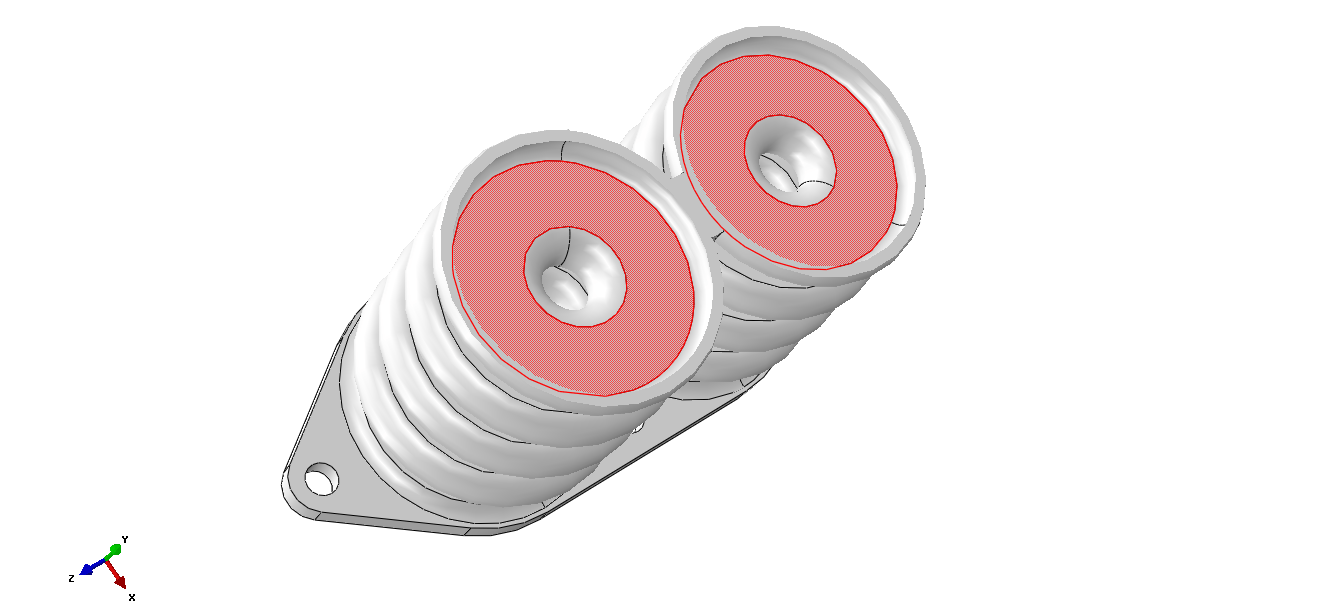
\includegraphics[width = \textwidth]{Figures/Chapter3/area.png}
    \caption{The red areas indicated the estimated area on which the pressure acts in y-direction}
    \label{fig4:bellowarea}
\end{figure}

This results in the following pressure mapping,

\begin{equation}
    \tau(p) = pA = 9048.64\cdot 10^{-6}p
\end{equation}

A bellow pressure of 80 $kPa$ will therefore result in a force of $724 N$. (Which is way to high, considering the flexibility when I held in my hands, a force of 7.24 Newton would be more on its place I think). Another way to find a pressure mapping is to introduce an effective surface area $A_{eff}$ which can be determined by attaching masses to the robot and measure elongation.



\subsection{Rotational stiffness determination}

In order to determine rotational stiffness of the robot, one bellow is inflated whilst the other bellow is not pressurized. Due to symmetry properties the rotational stiffness is assumed to be equal for both rotations. Figure (\ref{fig4:undeformed}) and (\ref{fig4:deformed}) show the undeformed and deformed soft robot for a single bellow pressure of 60 kPa. 


\begin{figure}[H]
\centering
\begin{minipage}{.5\textwidth}
  \centering
  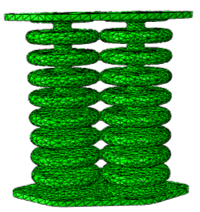
\includegraphics[width=0.6\linewidth]{Figures/Chapter3/singlesideundeformed60kPa.png}
  \captionof{figure}{Undeformed}
  \label{fig4:undeformed}
\end{minipage}%
\begin{minipage}{.5\textwidth}
  \centering
  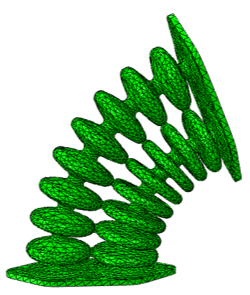
\includegraphics[width=0.65\linewidth]{Figures/Chapter3/singlesideddeformed60kPa.png}
  \captionof{figure}{Deformed, applying 60kPa on the left bellow}
  \label{fig4:deformed}
\end{minipage}
\end{figure}

In order to decouple elongation stiffness and rotational stiffness, post processing is necessary. This is done by extracting the nodes of interest, which are situated along the centre line of the robot. Tracking these nodes results in a cluster of nodes. This clusters of nodes can be used to fit the inverse kinematic model, as is done in Figure (\ref{fig4:midnodesfit}). In this way elongation and rotation can be separated in modal coordinates. Since the elongation stiffness is know, the rotational stiffness can be isolated. This has not succeeded yet.


\begin{figure}[H]
    \centering
    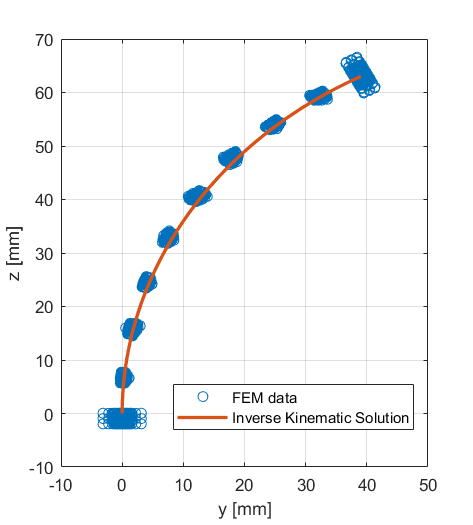
\includegraphics[width = 0.6\textwidth]{Figures/Chapter3/kinfit.png}
    \caption{Node clusters from FEM simulation and the fitted inverse kinematic solution}
    \label{fig4:midnodesfit}
\end{figure}

The inverse kinematic solution provides the generalized coordinates $q$ so the rotational and elongation contribution can be separated. At this point, this process still needs to be automated, now the fitting is done by hand. Additionally, a method still needs to found to decouple $K_{\theta}$ and $K_{yy}$.




